\chapter{Реализация} \label{chapt3}

Реализацию индекса можно декомпозировать на несколько частей:
\begin{itemize}
	\item Битовый массив (bit array)
	\item Логика z-order curve
	\item Встраивание в движок БД
	\item Lua-frontend
\end{itemize}

\section{Bit array}
Как описано в предыдущих пунктах, индексируемое значение получается
в результате перемешивания битов указанных индексируемых полей.
Данную структуру будем называть битовый массив. При реализации прототипа
было решено найти и использовать готовую реализацию на языке С.
Реализация была найдена --- \url{https://github.com/noporpoise/BitArray},
она удовлетворяла необходимым функциональным потребностям, однако имела
достаточно небольшое покрытие тестами, содержала баги, которые пришлось
исправить --- \url{https://github.com/noporpoise/BitArray/pull/15} и
была достаточно неоптимальной с учетом специфики решаемой задачи.

С учетом того, что для хранения и представления
большинства типов используется $64$ бита, размер массива всегда будет
кратен $64$ элементам. А именно $N * 64$, где $N$ --- количество частей
в индексе. Приведенная выше реализация содержала достаточно большое
число проверок и занимала больше памяти из-за того,
что являлось массивом общего назначения с возможностью динамического
изменения размера.
Для достижения максимальной эффективности пришлось реализовать свой
битовый массив постоянного размера и более оптимально работающий с
памятью (для выделения памяти использовалось 2 системных вызова,
один --- выделение структуры со служебными полями, другой сам массив).
В полученной реализации создание массива --- одна аллокация.
Служебное поле "количество элементов в массиве" также потеряло смысл
и было удалено поскольку вычисляется как $N * 64$.

Следующий шаг в оптимизации --- <<векторизация>>.
Большинство современных процессоров поддерживает так называемые
векторные инструкции, служащие для обработки массивов данных
(SIMD --- — Single Instruction Multiple Data).
По словам разработчиков использование таких инструкций позволяет
получать прирост производительности до 30\%.
О том, что какой-то цикл может быть векторизован можно с
помощью директивы \textit{\#pragma simd},
однако это не дает гарантий, что цикл будет векторизован,
компилятор может и проигнорировать данную директиву, к тому же
большинство современных компиляторов могут автоматически находить
векторизуемые циклы. Посмотреть за тем, векторизуется цикл или нет,
можно с помощью специальных опций компилятора.

Циклы для операций AND и OR были векторизованы для компиляторов
GCC v7.4.0 и Apple Clang v11.0.0.

\subsection{Bit interleaving}
Поскольку одной из ключевых операций является перемешивание битов, эта функциональность была добавлена для битового массива.

Вычисление производится не тривиальным образом, а с помощью так называемых lookup-таблиц. Таблица ставит в соответствие любому числу от 0 до 255 значение, вычисляемое по правилу $\sum{i=0}^7(k_i * 2^{i*n})$, где $n$ - число массивов, которые должны быть перемешаны, $k_i$ - значение $i$-ого бита. Для каждой части в зависимости от её номера m хранится сдвинутая на m разрядов копия такой lookup-таблицы.

Соответственно вычисление z-адреса происходит за $8*n$ обращений, сдвигов и применения логической операции $OR$, где n - число массивов. Стоит обратить внимание, что lookup-таблицы вычислены для октетов, а не больших размеров. Использование для $n=16/32/64$ значений затруднено, поскольку расходы памяти на хранение этой таблицы растут экспоненциально как $~2^n$.


\section{Z-order curve}
Изначально информация о существовании индекса на основе кривой z-порядка была получена из статей Amazon~\cite{DynamoZorderP1, DynamoZorderP2}, данные статьи являются скорее инструкцией для пользователей, как создать индекс на основе кривой Мортона для удовлетворения пользовательских потребностей с минимальными накладными расходами (z-order curve не является встроенной функциональностью DynamoDB).

Основные идеи, которые можно было бы почерпнуть из статьи --- алгоритмы работы с кривой z-порядка и работа с различными типами данных - необходимо найти функцию, которая для каждого типа данных возвращает битовую строку. Для различных значений битовые строки должны быть лексикографически упорядочены. Например, рассмотрим знаковые целые числа $-1$ и $2$. Для них выполняется следующее неравенство $-1 < 2$. Однако в бинарном представлении $-1$ --- это $11111111$, а 2 --- $00000010$. Лексикографический порядок нарушен. Для восстановления предлагается инвертировать старший бит, тогда значения для $-1$ --- $01111111$ и $10000010$ для $2$. Другие типы будут рассмотрены в следующей главе.

После вычисления z-адреса для каждого проиндексированного значения и размещения его в B-дереве мы получаем структуру, из которой хотелось бы выбирать значения, соответствующие нашим запросам. Самое первое, что может определить пользователь - нижнюю и верхнюю границы поиска (lower и upper bound). Рассмотрим пример для случая двух измерений. Мы хотим сделать выборку в прямоугольнике $[x_{min};x_{max}]$ и $[y_{min}; y_{max}]$ - границами будут $z\_address(x_{min}, y_{min})$ и $z\_address(x_{max}, y_{max})$. В интервал между двумя этими значениями может попадать достаточно большое число значений, не принадлежащих заданному прямоугольнику. Перед тем как объяснять алгоритм итерации по данной структуре следует ввести 2 ключевые функции - $is\_relevant(lower\_bound, upper\_bound, z\_address)$, которая проверяет $z\_address$ на принадлежность заданному прямоугольнику, и $next\_jump\_in(lower\_bound, upper\_bound, z\_address)$, возвращающая для z-адреса за пределами прямоугольника первое по порядку значение, попадающее в прямоугольник.
С учетом вышесказанного итерация выглядит следующим образом. Мы начинаем с некоторого $z\_address$ значения (большего или равного $lower\_bound$), проверяем его принадлежность прямоугольнику с помощью  $is\_relevant$, если функция вернула $true$, то это значение возвращается пользователю, иначе с помощью $next\_jump\_in$ переходим к следующему подходящему значению, пока не выйдем за границу $upper\_bound$.

Описание двух, используемых выше алгоритмов, можно найти в~\cite{ramsak2000integrating, widhopf2005advanced, prukl2007relavcni} С некоторыми изменениями и модификациями они были реализованы в рамках дипломной работы. Например, функция $is\_relevant$ может рассматриваться как часть функции $next\_jump\_in$ и практически без изменений извлечена в отдельную функцию. Однако такой наивный подход неоптимален, функцию можно упростить, добавить дополнительные оптимизации и применить эвристики, способные ускорить данные функции.
Во-первых, там, где можно было отказаться от массивов в пользу битовых масок, это было сделано.
Как было сказано, ключ --- это массив 64-битных чисел, однако если индексируемые числа небольшие, то большая часть битов будет нулевой.
Приведенные алгоритмы проверки и поиска работают за $O(N)$, где N ---
длина ключа. При этом если биты с одинаковым порядковым номером $z\-value$, $lower\ bound$ и $upper\ bound$ могут быть безболезненно
пропущены, это же справедливо и для более крупных единиц, например, байтов. Данная эвристика для размерности $3$ и чисел из интервала $[0; 255]$ дала выигрыш $15-20\%$.

Отдельно стоит отметить более рациональных подход к используемым типам данных.
Использование типов как можно меньшей размерности, скажем,
$uint8\_t$ вместо $uint64\_t$ дало существенный прирост производительности, сократив время работы функций практически в 2 раза.

\section{Tarantool index}
В терминах ООП --- индекс это класс, обладающий некоторым набором функций и реализующий некоторую структуру данных, хранящую информацию о проиндексированных кортежах.
Как было описано в предыдущих частях, вычисленные z-адреса сохраняются в B-дереве. В СУБД Tarantool уже была готовая реализация B+*-tree, которую было решено переиспользовать.

СУБД Tarantool имеет собственную систему типов. Для индекса было выбрано несколько поддерживаемых типов - unsigned (unsigned integer), integer (signed integer), number (double-precision floating-point number) и string (только префиксный поиск по первым 64 битам). Это достаточно сильно отличает данный индекс от уже существующего R-Tree, предназначенного для работы с числами с плавающей точкой. 

Как было сказано, для корректной работы нужно научиться преобразовывать значения определенного типа к некоторым битовым лексикографически упорядоченным словам. Все указанные типы используют 64 бита для хранения, соответствующие им значения решено было хранить как unsigned integer размером 64 бита. 

Для unsigned integer преобразование является тривиальным, поскольку в битовые представления и так лексикографически упорядочены. 

У знаковых целых чисел (signed integers) старший бит является меткой знака. То есть с точки зрения бинарного представления любое отрицательное число больше любого положительного. Получить значение, удовлетворяющее нужным критериям можно с помощью инверсии старшего бита.

Поиск по строкам, как было сказано, возможен только префиксный. Первые 8 байт любой строки сохраняются как unsigned integer число, в случае если строка короче, она дополняется нулями в конце. Если используется строка в кодировке ASCII, то значения будут уже лексикографически отсортированы. Кодировка UTF-8 обратно совместима с ASCII, поэтому также может использоваться. Такой подход исключает поддержку collation’ов. Но всё-таки поддержку данного типа было решено оставить, поскольку 8 байт может быть вполне достаточно для многих пользовательских сценарий. Кроме того, данный поиск можно использовать как первичный, и при необходимости пользователь сам может выполнить дополнительную фильтрацию.

Наиболее сложный для рассмотрения вариант --- числа с плавающей точкой двойной точности (double).
Для того, чтобы разобраться с этим случаем следует обратиться к спецификации IEEE 754,
говорящего что “если два числа с плавающей запятой одного и того же формата упорядочены (скажем, x < y),
то они упорядочиваются таким же образом, когда их биты интерпретируются как целые числа со знаками (sign-magnitude integers)”.
Нужное нам преобразование имеет следующий вид: для положительных чисел инвертируется старший бит, для отрицательных инвертируются все биты.

Отдельно стоит отметить $null$-значения. Они не поддерживаются в силу того, что невозможно задать битовое значение, которое бы соответствовало бы отсутствию любого значения.
Однако в пользовательском интерфейсе можно будет использовать такие значение для задания минимально возможного и максимально возможного значения ключа. Но это будет рассмотрено в следующих частях.

В реляционных базах данных индексы могут быть уникальными (индекс может содержать один экземпляр определенного значения) и неуникальными. Для Tarantool это тоже справедливо. Предполагается,что  для каждого спейса (аналог реляционной таблицы) определен как минимум один индекс. Самый первый индекс должен быть уникальным и называется первичным. Именно в качестве первичного ключа предлагается использовать z-order curve по задумке авторов стать Amazon. Однако в нашем случае было решено поступить иначе, запретить делать индекс на основе кривой z-порядка уникальным.

Любой индекс предполагает, что элементы внутри него располагаются детерминировано при построении при запуске, вставке очередного элемента и т.д. При появлении неуникальных значений встает вопрос о том, как сортировать эти значения. В Tarantool принято сортировать неуникальные вторичные ключи путем дописывания первичного ключа. Полученный ключ является уникальным и обычно не возникает проблем с сортировкой таких значений. Рассмотрим подробнее, как эта проблема была решена. Начнем с того, как это делается для B-Tree индекса. Вспомним, что кортеж (tuple) - это массив значений, закодированных в формат MessagePack. Для каждого индекса определены 2 значения $key\_def$ - поля, входящие в индекс, и $cmp\_def$ --- $key\_def$, расширенный первичным ключом, а значит уникальный. Это не банальное дописывание первичного ключа в конец, это добавление полей, отсутствующих в $key\_def$, т.е. каждое поле может встретится только один раз в $key\_def$ и $cmp\_def$. $key\_def$ виден пользователю, однако в самом дереве хранится значение, соответствующее расширенному ключу. Сравнение двух кортежей производится с учетом полей, перечисленных в $cmp\_def$’e.

Таким образом работу с индексом можно описывать как независимые 2 части ---
чтение и запись.
Алгоритм записи следующий:
\begin{itemize}
	\item Извлечь из полученного кортежа его z-адрес;
	\item Вставить в дерево элемент --- структуру, состоящую из z-адреса и указателя на кортеж.
\end{itemize}

Алгоритм чтения:
\begin{itemize}
	\item Извлечь z-адрес из ключа поиска;
	\item Получить итератор на наименьший элемент с таким ключом;
	\item Последовательно итерироваться по дереву, проверяя каждый элемент на принадлежность к региону поиска;
	\item В случае выхода за границу сделать прыжок для возврата в регион поиска;
	\item Прекратить поиск, если очередной элемент больше, чем $upper\_bound$.
\end{itemize}

\section{Lua frontend}
Приводится описание того, как конечный пользователь должен выполнять
запрос к базе данных с целью сохранения, поиска, удаления и модификации
какого-либо элемента.

\begin{lstlisting}
-- Создание space "test" - аналога таблицы в реляционных БД
local space = box.schema.space.create('test',
	{ engine = 'memtx' })
-- Создание первичного ключа
local pk = space:create_index('pk', 
	{ type = 'tree', parts = {{1, 'unsigned'}}})
-- Создание индекса на основе z-order curve
-- Индексируемые поля 2 типа "unsigned" и 3 типа "integer"
local sk = space:create_index('secondary',
	{ type = 'zcurve', parts = {{2, 'unsigned'}, {3, 'integer'}}})
-- Вставка кортежа {1, 2, 3} в space
space:replace({1, 2, 3})
-- Прибавление ко второму полю кортежа единицы
space:update({1}, {{'+', 2, 1}})
-- Удаление кортежа
space:delete({1})
-- Выборка по всему индексу
sk:select()
sk:select({}, {iterator = 'ALL'})
-- Выборка в интервале от [0; 2] и [3; 5]
sk:select({0, 2, 3, 5})
sk:select({0, 2, 3, 5}, { iterator = 'EQ' })
sk:select({0, 2, 3, 5}, { iterator = 'GE' })
-- Выборка значений {5; 6}
sk:select({5, 6})
sk:select({5, 6}, {iterator = 'EQ'})
-- Выборка значений [5; +inf] и [6; +inf]
sk:select({5, 6}, {iterator = 'GE'})
-- Выборка значений [-inf; 5] и [-inf; +inf]
sk:select({box.NULL, 5, box.NULL, box.NULL}, {iterator = 'GE'})
-- Удаление индекса
sk:drop()
\end{lstlisting}
Как видно, индекс поддерживает 3 итератора <<ALL>> --- выборка всех данных,
<<EQ>> - выборка данных с указанным ключом и <<GE>> - выборка данных, больше либо равных указанному ключу.

<<box.NULL>> --- специальный символ, указывающий на отсутствие значения. Если он стоит на нечетном месте, то эквивалентен $-\infty$, на чётном --- $+\infty$.

\chapter{Результаты} \label{chapt4}
Было проведено несколько тестов:
\begin{itemize}
	\item Сравнение с R-Tree --- поиск точек внутри гиперкуба
	размерности от 1 до 20;
	\item Сравнение с B-Tree --- поиск точек внутри гиперкуба
	размерности от 1 до 20;
	\item Сравнение с B-Tree --- префиксный поиск.
\end{itemize}

В каждом из тестов отдельно интересуют значения времени, потраченного на вставку тестового датасета, время выполнения запросов
и объем потребляемой памяти.

Также будет проверено 3 варианта распределения значений в пространстве.
В первом случае запрос будет делаться за данными, распределенными равномерно.
Т.е. координаты точек --- случайно распределенные числа в некотором интервале $[V_{min}; V_{max}]$.
Во втором случае запрос должен будет вернуть пустое множество --- данных удовлетворяющих
запросу нет.
И в последнем случае запрос будет высокоселективным,
данные будут сконцентрированы вблизи одной точки,
больший вклад во время выполнения запроса начнет давать не только время поиска нужных данных,
но и время десериализвации результатов перед возвратом клиенту.

\section{Сравнение с R-Tree. Поиск точек внутри гиперкуба}

\subsubsection{Описание среды и условий проведения измерений}

Для каждого из тестов создавались 2 спейса,
содержащих 2 индекса --- первичный B-Tree и вторичный R-tree или Z-order curve. Последовательно в каждый из спейсов вставлялись приготовленные кортежи,
измерялось время вставки и память, которую занимает индекс
Стоит отметить, что для ускорения вставки и исключения факторов,
способных её замедлить, были отключены WAL (Write-ahead logs) ---
запись всех операций в специальный журнал, предотвращающий потерю данных в случае перезагрузки или остановки СУБД.
После чего производилось $N_{q}$ запросов,
и измерялось время, за которое они все были исполнены.

В первом случае равномерного распределения генерировалось $10^6$ значений в интервале
от $0$ до $10^5$.
Область запроса --- интервал $[0.35 \times v_{max}; 0.75 \times v_{max}]$ по каждой из размерностей, $v_{max}$ --- максимально сгенерированное случайное значение. Для усреднения результатов каждый из запросов повторялся 10 раз.

% XXX: empty queries

В случае высокоселективной выборки случайным образом для размерности $D$ генерировались значения $v_i$ в диапазоне от $0$ до $V = 2.5 \times 10^8$ при этом большая часть значений лежит около 0,
ими заполнялись 2 кортежа --- для R-Tree (с массивом: $\{id, \{v_1, v_2, ..., v_D\}\}$) и для Z-Order curve (без массива: $\{id, v_1, v_2, ..., v_D\}$). $id$ - первичный ключ, число типа unsigned.
Всего $N_{t} = 10^6$ значений.

Далее генерировалось 2 числа $Q_{min}$ и $Q_{max}$ ($Q_{min} < Q_{max}$) для ограничения области в пространстве $[Q_{min}; Q_{max}]$ в каждой размерности $N_{q} = 10^3$ пар.

\subsubsection{Результаты}

\begin{figure}
	\centering
	\label{img:insert_rtree_normal}
	\caption{Сравнение скорости вставки в R-Tree и Z-order curve индексы}
	\begin{tikzpicture}
	% Package PGFPLOTS manual p.84
	\begin{axis}[
	ybar,
	legend style={at={(0.5,-0.1)},
		anchor=north,legend columns=-1},
	ylabel={Время вставки в секундах},
	xlabel={Размерность},
	symbolic x coords={1, 2, 3, 5, 10, 15, 18, 20},
	xtick=data,
	nodes near coords,
	nodes near coords align={vertical},
	width  = \textwidth,
	enlarge x limits  = 0.1,
	scaled y ticks = false,
	]
	\addplot +[bar shift=-12pt] coordinates {
		(1,2.1)
		(2,0.9)
		(3,0.21)
		(5,0.04)
		(10,0.05)
		(15,0.09)
		(18,0.2)
		(20,0.24)
	};
	\addplot +[bar shift=+12pt] coordinates {
		(1,2.3)
		(2,1.2)
		(3,0.44)
		(5,0.35)
		(10,0.41)
		(15,0.10)
		(18,0.04)
		(20,0.02)
	};
	\legend{R-Tree, Z-order curve}
	\end{axis}
	\end{tikzpicture}
\end{figure}

\begin{figure}
	\centering
	\label{img:insert_rtree_normal_selection}
	\caption{Селективность запросов в случае равномерно распределенных значений}
	\begin{tikzpicture}
	% Package PGFPLOTS manual p.84
	\begin{axis}[
	ybar,
	legend style={at={(0.5,-0.1)},
		anchor=north,legend columns=-1},
	xlabel={Размерность},
	symbolic x coords={1, 2, 3, 5, 10, 15, 18, 20},
	xtick=data,
	nodes near coords,
	nodes near coords align={vertical},
	width  = \textwidth,
	enlarge x limits  = 0.1,
	scaled y ticks = false,
	]
	\addplot +[bar shift=+12pt] coordinates {
		(1,399491)
		(2,159021)
		(3,63951)
		(5,10181)
		(10,95)
		(15,2)
		(18,0)
		(20,0)
	};
	\legend{Количество значений}
	\end{axis}
	\end{tikzpicture}
\end{figure}

\begin{figure}
\centering
\label{img:insert_rtree}
\caption{Сравнение скорости вставки в R-Tree и Z-order curve индексы}
\begin{tikzpicture}
% Package PGFPLOTS manual p.84
\begin{axis}[
ybar,
legend style={at={(0.5,-0.1)},
	anchor=north,legend columns=-1},
ylabel={Время вставки в секундах},
xlabel={Размерность},
symbolic x coords={1, 2, 3, 5, 10, 15, 18, 20},
xtick=data,
nodes near coords,
nodes near coords align={vertical},
width  = \textwidth,
enlarge x limits  = 0.1,
scaled y ticks = false,
]
\addplot +[bar shift=-12pt] coordinates {
	(1,1.95)
	(2,2.43)
	(3,3.21)
	(5,3.96)
	(10,6.20)
	(15,8.84)
	(18,9.91)
	(20,10.76)
};
\addplot +[bar shift=+12pt] coordinates {
	(1,2.19)
	(2,2.53)
	(3,2.82)
	(5,3.46)
	(10,4.41)
	(15,4.94)
	(18,5.41)
	(20,5.71)
};
\legend{R-Tree, Z-order curve}
\end{axis}
\end{tikzpicture}
\end{figure}

\begin{figure}
\centering
\label{img:mem_rtree}
\begin{tikzpicture}
% Package PGFPLOTS manual p.84
\begin{axis}[
ybar,
legend style={at={(0.5,-0.1)},
	anchor=north,legend columns=-1},
ylabel={Потребляемая память в мегабайтах},
xlabel={Размерность},
symbolic x coords={1, 2, 3, 5, 10, 15, 18, 20},
xtick=data,
nodes near coords,
nodes near coords align={vertical},
width  = \textwidth,
enlarge x limits  = 0.1,
restrict y to domain=0:500,
]
\addplot +[bar shift=-10pt] coordinates {
	(1, 36)
	(2, 60)
	(3, 85)
	(5, 129)
	(10, 245)
	(15, 352)
	(18, 425)
	(20, 475)
};
\addplot +[bar shift=+10pt] coordinates {
	(1, 34)
	(2, 41)
	(3, 49)
	(5, 64)
	(10, 102)
	(15, 141)
	(18, 163)
	(20, 179)
};
\legend{R-Tree,Z-order curve}
\end{axis}
\end{tikzpicture}
\end{figure}

\begin{figure}
\centering
\begin{tikzpicture}
\label{img:select_rtree}
% Package PGFPLOTS manual p.84
\begin{axis}[
ybar,
legend style={at={(0.5,-0.1)},
	anchor=north,legend columns=-1},
ylabel={Время выборки в секундах},
xlabel={Размерность},
symbolic x coords={1, 2, 3, 5, 10, 15, 18, 20},
xtick=data,
nodes near coords,
nodes near coords align={vertical},
width  = \textwidth,
enlarge x limits  = 0.1,
]
\addplot +[bar shift=-10pt] coordinates {
	(1, 358.5)
	(2, 204.3)
	(3, 131.0)
	(5, 46.6)
	(10, 18.7)
	(15, 21.7)
	(18, 21.7)
	(20, 22.9)
};
\addplot +[bar shift=+10pt] coordinates {
	(1, 383.7)
	(2, 217.4)
	(3, 160.1)
	(5, 107.7)
	(10, 216.2)
	(15, 531.8)
	(18, 847.1)
	(20, 1156.9)
};
\legend{R-Tree,Z-order curve}
\end{axis}
\end{tikzpicture}
\end{figure}

Дадим интерпретацию полученным результатам. Во-первых, как видно
из рис.~\ref{img:insert_rtree} скорость вставки в Z-order curve индекс выше, чем в R-Tree. Данный тренд сохраняется и при увеличении размерности. На практике однако результат не особо релевантен,
поскольку, как было отмечено выше, тест проводился с выключенным WAL.

С точки зрения расхода памяти оптимальнее Z-order curve.
Причем на больших размерностях практически в три раза.
Это уже можно считать релевантным положительным результатом, поскольку
объем оперативной памяти обычно ограничен. С другой стороны,
её стоимость постоянно снижается.

Последний график, показывающий время выполнения запросов на чтение наиболее интересен.
Как видно примерно до размерности 5 время уменьшается,
после чего для R-Tree остается практически постоянным, а для Z-order
curve начинает драматически возрастать.
Дело в том, что при одинаковом количестве точек с увеличением размерности
начинает падать селективность наших запросов. Больше размерностей ---
меньше вероятность того, что координаты точки попадут в интервал между
границами запроса. Для R-Tree низкая селективность некритична,
поэтому в конце время выполнения запросов практически одинаково.
Совершенно иначе обстоит дело с Z-order Curve
Как только итератор натыкается на точку, лежащую вне границ поиска
вычисляется Z-адрес следующего вхождения в указанную область.
После этого совершается прыжок --- спуск по дереву в эту точку.
Если данной точки не существует, то мы попадем в следующую по порядку.
Данная точка снова может лежать вне области поиска, тогда ситуация будет повторяться вновь и вновь. Это обоснование правой части графика.
Слева при высокой селективности большая часть времени может тратится
не на сам поиск, а на то, чтобы упаковать данные и вернуть их клиенту.
При работе с внешними коннекторами --- это пересылка по сети,
при доступе из Lua-приложения это дополнительная работа по сериализации/десериализации Lua-объектов перед возвратом пользователю.
Также, если при спуске по R-дереву понять принадлежность точки/области гиперкубу 
можно за количество операций, зависящих от размерности,
то при работе с Z-адресами алгоритмы линейно зависят от длины этого адреса ---
размерность, умноженная на достаточно большую константу --- 64.

\section{Сравнение с B-Tree. Поиск точек внутри гиперкуба}

\subsubsection{Описание среды и условий проведения измерений}
В первом случае генерируется $10^6$ значений равномерно распределенных в интервале $[0; 10^5]$.
Область запроса --- интервал $[0.35 \times v_{max}; 0.75 \times v_{max}]$ по каждой из размерностей, $v_{max}$ --- максимально сгенерированное случайное значение. Для усреднения результатов каждый из запросов повторялся 10 раз.

\begin{figure}
	\centering
	\begin{tikzpicture}
	\label{img:select_btree_normal}
	% Package PGFPLOTS manual p.84
	\begin{axis}[
	ybar,
	legend style={at={(0.5,-0.1)},
		anchor=north,legend columns=-1},
	ylabel={Время выборки в секундах},
	xlabel={Размерность},
	symbolic x coords={1, 2, 3, 5, 10, 15, 18, 20},
	xtick=data,
	nodes near coords,
	nodes near coords align={vertical},
	width  = \textwidth,
	enlarge x limits  = 0.1,
	]
	\addplot +[bar shift=-10pt] coordinates {
		(1, 8.0)
		(2, 6.4)
		(3, 7.5)
		(5, 5.1)
		(10, 11.6)
		(15, 11.6)
		(18, 13.7)
		(20, 12.5)
	};
	\addplot +[bar shift=+10pt] coordinates {
		(1, 5.1)
		(2, 1.6)
		(3, 0.5)
		(5, 0.4)
		(10, 0.4)
		(15, 0.1)
		(18, 0.04)
		(20, 0.05)
	};
	\legend{B-Tree,Z-order curve}
	\end{axis}
	\end{tikzpicture}
\end{figure}

\begin{figure}
	\centering
	\begin{tikzpicture}
	\label{img:select_btree_normal_selection}
	% Package PGFPLOTS manual p.84
	\begin{axis}[
	ybar,
	legend style={at={(0.5,-0.1)},
		anchor=north,legend columns=-1},
	ylabel={Селективность тестовых запросов, количество кортежей},
	xlabel={Размерность},
	symbolic x coords={1, 2, 3, 5, 10, 15, 18, 20},
	xtick=data,
	nodes near coords,
	nodes near coords align={vertical},
	width  = \textwidth,
	enlarge x limits  = 0.1,
	]
	\addplot +[bar shift=-10pt] coordinates {
		(1, 399491)
		(2, 159021)
		(3, 63951)
		(5, 10181)
		(10, 95)
		(15, 2)
		(18, 0)
		(20, 0)
	};
	\legend{Количество значений}
	\end{axis}
	\end{tikzpicture}
\end{figure}

% XXX: empty queries

Для высокоселектиных запросов, как и при сравнении с R-Tree, генерировалось $N = 10^6$ значений.
В том же диапазоне от $0$ до $2.5 \times 10^8$, однако большая из часть сконцентрирована в районе 0.
Значения вставлялись в один спейс, в котором были созданы три индекса ---
первичный уникальный ключ, B-Tree индекс по первому полю и Z-order curve по второму и всем последующим полям.
Далее выбирались точки из гиперкуба в интервале $[1; v_{max}/4]$, где $v_{max}$ --- самое большое
сгенерированное значение.
Чтобы избежать случайных выбросов и усреднить результаты, каждый запрос был сделан 10 раз.

\subsubsection{Результаты и интерпретация}
Результаты с нормальным распределением приведены на рисунке~\ref{img:select_btree_normal_selection}.
Как и ожидалось, Z-order curve показал себя быстрее, чем B-Tree.
Время, которое тратилось на сканирование значений, не входящих в интервал поиска,
значительно превышало время, которое затрачивалось на вычисление $next_intersection_point$
в случае выхода за границу поиска и прыжка к этой точке.
При этом заметим, что результаты, полученные для больших размерностей не являются особо показательными,
поскольку значений, удовлетворяющих критериям запроса было либо слишком мало,
либо совсем не было.

Результаты приведены на рисунке~\ref{img:select_btree_highselective}
\begin{figure}
	\centering
	\begin{tikzpicture}
	\label{img:select_btree_highselective}
	% Package PGFPLOTS manual p.84
	\begin{axis}[
	ybar,
	legend style={at={(0.5,-0.1)},
		anchor=north,legend columns=-1},
	ylabel={Время выборки в секундах},
	xlabel={Размерность},
	symbolic x coords={1, 2, 3, 5, 10, 15, 18, 20},
	xtick=data,
	nodes near coords,
	nodes near coords align={vertical},
	width  = \textwidth,
	enlarge x limits  = 0.1,
	]
	\addplot +[bar shift=-10pt] coordinates {
		(1, 22.6)
		(2, 12.6)
		(3, 23.4)
		(5, 21.7)
		(10, 17.3)
		(15, 24.5)
		(18, 21.9)
		(20, 21.9)
	};
	\addplot +[bar shift=+10pt] coordinates {
		(1, 10.0)
		(2, 11.2)
		(3, 12.5)
		(5, 17.0)
		(10, 16.6)
		(15, 19.5)
		(18, 24.2)
		(20, 24.8)
	};
	\legend{B-Tree,Z-order curve}
	\end{axis}
	\end{tikzpicture}
\end{figure}

В графиках присутствуют выбросы, но общая тенденция видна --- при высокоселективных запросах
использование Z-order curve оправдано.
Однако с увеличением размерности и уменьшением селективности
сканирование начинает быть эффективнее, чем частые спуски по дереву для пропуска интервала,
не входящего в область запроса.

\section{Сравнение с B-Tree. Префиксный поиск}

\begin{figure}[ht] 
	\centering
	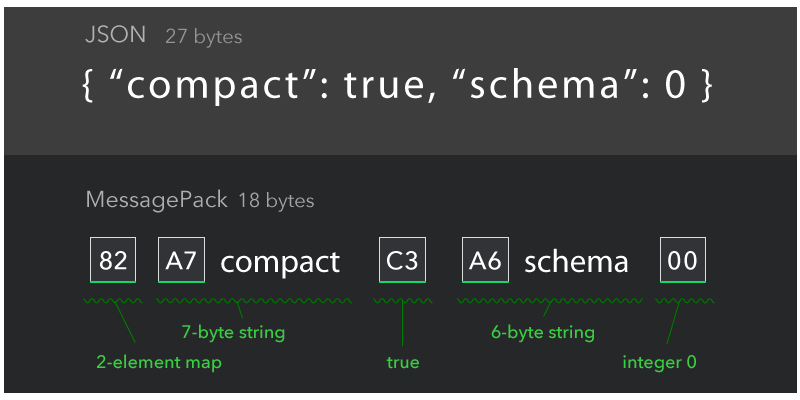
\includegraphics [scale=0.4] {message-pack.png}
	\caption{Сравнение хранения в JSON-формате (plain text). И message pack (binary)}
	\label{img:msgpack}
\end{figure}

Поиск производился по спейсу, заполненную одинаковыми строками.
Выполнялся запрос с итератором <<EQ>> --- equal.
B-дерево оказалось медленнее примерно на $15\%$.
Это связано с тем, что существующая реализация не использует дополнительной памяти
для хранения проиндексированных значений.
Поэтому каждая итерация --- это декодинг message pack (см. рис~\ref{img:msgpack},~\cite{messagepack_site})
строки и затем уже сравнение.
В противоположность Z-order curve индекс хранит дополнительно 8 байт
на каждое проиндексированное значение.
Декодирования на каждой итерации не происходит, что и является причиной подобного
прироста производительности.
